\documentclass{standalone}
\usepackage{tikz}
\usetikzlibrary{patterns, positioning}


\begin{document}
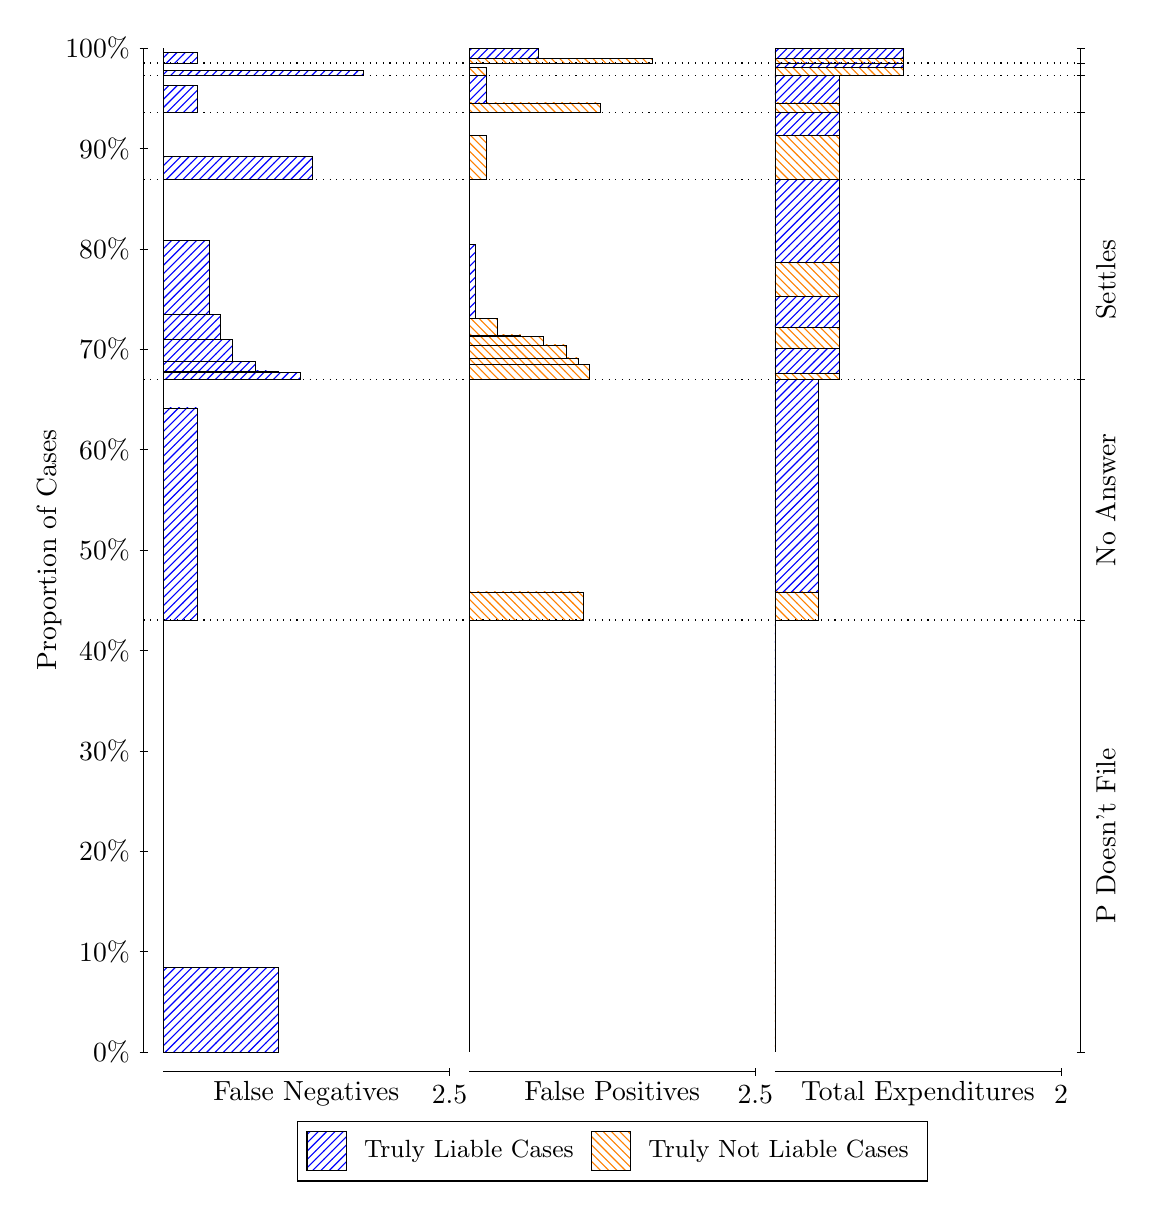
\begin{tikzpicture}
\draw[black, very thin] (1.5,1.75) -- (1.5,14.5);
\node[rotate=90, text=black, anchor=center] at (0.3, 8.125) {Proportion of Cases};
\draw[black, very thin] (1.45,1.75) -- (1.55,1.75);
\node[text=black, anchor=east] at (1.45, 1.75) {0\%};
\draw[black, very thin] (1.45,3.025) -- (1.55,3.025);
\node[text=black, anchor=east] at (1.45, 3.025) {10\%};
\draw[black, very thin] (1.45,4.3) -- (1.55,4.3);
\node[text=black, anchor=east] at (1.45, 4.3) {20\%};
\draw[black, very thin] (1.45,5.575) -- (1.55,5.575);
\node[text=black, anchor=east] at (1.45, 5.575) {30\%};
\draw[black, very thin] (1.45,6.85) -- (1.55,6.85);
\node[text=black, anchor=east] at (1.45, 6.85) {40\%};
\draw[black, very thin] (1.45,8.125) -- (1.55,8.125);
\node[text=black, anchor=east] at (1.45, 8.125) {50\%};
\draw[black, very thin] (1.45,9.4) -- (1.55,9.4);
\node[text=black, anchor=east] at (1.45, 9.4) {60\%};
\draw[black, very thin] (1.45,10.675) -- (1.55,10.675);
\node[text=black, anchor=east] at (1.45, 10.675) {70\%};
\draw[black, very thin] (1.45,11.95) -- (1.55,11.95);
\node[text=black, anchor=east] at (1.45, 11.95) {80\%};
\draw[black, very thin] (1.45,13.225) -- (1.55,13.225);
\node[text=black, anchor=east] at (1.45, 13.225) {90\%};
\draw[black, very thin] (1.45,14.5) -- (1.55,14.5);
\node[text=black, anchor=east] at (1.45, 14.5) {100\%};

\draw[black, very thin] (13.4,1.75) -- (13.4,14.5);
\draw[black, very thin] (13.35,1.75) -- (13.45,1.75);
\node[anchor=west] at (13.35, 1.75) {};
\draw[black, very thin] (13.35,7.2363) -- (13.45,7.2363);
\node[anchor=west] at (13.35, 7.2363) {};
\draw[black, very thin] (13.35,10.287) -- (13.45,10.287);
\node[anchor=west] at (13.35, 10.287) {};
\draw[black, very thin] (13.35,12.835) -- (13.45,12.835);
\node[anchor=west] at (13.35, 12.835) {};
\draw[black, very thin] (13.35,13.678) -- (13.45,13.678);
\node[anchor=west] at (13.35, 13.678) {};
\draw[black, very thin] (13.35,14.154) -- (13.45,14.154);
\node[anchor=west] at (13.35, 14.154) {};
\draw[black, very thin] (13.35,14.31) -- (13.45,14.31);
\node[anchor=west] at (13.35, 14.31) {};
\draw[black, very thin] (13.35,14.5) -- (13.45,14.5);
\node[anchor=west] at (13.35, 14.5) {};

\draw[black, very thin, pattern color=blue, pattern=north east lines] (1.75,1.75) rectangle (3.2033,2.8274);
\draw[black, very thin, pattern color=orange, pattern=north west lines] (1.75,2.8274) rectangle (1.75,7.2363);
\draw[black, very thin, pattern color=blue, pattern=north east lines] (1.75,7.2363) rectangle (2.186,9.9301);
\draw[black, very thin, pattern color=orange, pattern=north west lines] (1.75,9.9301) rectangle (1.75,10.287);
\draw[black, very thin, pattern color=blue, pattern=north east lines] (1.75,10.287) rectangle (3.494,10.379);
\draw[black, very thin, pattern color=blue, pattern=north east lines] (1.75,10.379) rectangle (3.2033,10.394);
\draw[black, very thin, pattern color=blue, pattern=north east lines] (1.75,10.394) rectangle (3.058,10.401);
\draw[black, very thin, pattern color=blue, pattern=north east lines] (1.75,10.401) rectangle (2.9127,10.525);
\draw[black, very thin, pattern color=blue, pattern=north east lines] (1.75,10.525) rectangle (2.622,10.797);
\draw[black, very thin, pattern color=blue, pattern=north east lines] (1.75,10.797) rectangle (2.4767,11.114);
\draw[black, very thin, pattern color=blue, pattern=north east lines] (1.75,11.114) rectangle (2.3313,12.059);
\draw[black, very thin, pattern color=orange, pattern=north west lines] (1.75,12.059) rectangle (1.75,12.835);
\draw[black, very thin, pattern color=blue, pattern=north east lines] (1.75,12.835) rectangle (3.6393,13.126);
\draw[black, very thin, pattern color=orange, pattern=north west lines] (1.75,13.126) rectangle (1.75,13.678);
\draw[black, very thin, pattern color=blue, pattern=north east lines] (1.75,13.678) rectangle (2.186,14.028);
\draw[black, very thin, pattern color=orange, pattern=north west lines] (1.75,14.028) rectangle (1.75,14.154);
\draw[black, very thin, pattern color=blue, pattern=north east lines] (1.75,14.154) rectangle (4.2933,14.212);
\draw[black, very thin, pattern color=orange, pattern=north west lines] (1.75,14.212) rectangle (1.75,14.31);
\draw[black, very thin, pattern color=blue, pattern=north east lines] (1.75,14.31) rectangle (2.186,14.441);
\draw[black, very thin, pattern color=orange, pattern=north west lines] (1.75,14.441) rectangle (1.75,14.5);
\draw[black, very thin, pattern color=orange, pattern=north west lines] (5.6333,1.75) rectangle (5.6333,6.1589);
\draw[black, very thin, pattern color=blue, pattern=north east lines] (5.6333,6.1589) rectangle (5.6333,7.2363);
\draw[black, very thin, pattern color=orange, pattern=north west lines] (5.6333,7.2363) rectangle (7.0867,7.593);
\draw[black, very thin, pattern color=blue, pattern=north east lines] (5.6333,7.593) rectangle (5.6333,10.287);
\draw[black, very thin, pattern color=orange, pattern=north west lines] (5.6333,10.287) rectangle (7.1593,10.486);
\draw[black, very thin, pattern color=orange, pattern=north west lines] (5.6333,10.486) rectangle (7.014,10.566);
\draw[black, very thin, pattern color=orange, pattern=north west lines] (5.6333,10.566) rectangle (6.8687,10.731);
\draw[black, very thin, pattern color=orange, pattern=north west lines] (5.6333,10.731) rectangle (6.578,10.835);
\draw[black, very thin, pattern color=orange, pattern=north west lines] (5.6333,10.835) rectangle (6.4327,10.842);
\draw[black, very thin, pattern color=orange, pattern=north west lines] (5.6333,10.842) rectangle (6.2873,10.856);
\draw[black, very thin, pattern color=orange, pattern=north west lines] (5.6333,10.856) rectangle (5.9967,11.063);
\draw[black, very thin, pattern color=blue, pattern=north east lines] (5.6333,11.063) rectangle (5.706,12.008);
\draw[black, very thin, pattern color=blue, pattern=north east lines] (5.6333,12.008) rectangle (5.6333,12.835);
\draw[black, very thin, pattern color=orange, pattern=north west lines] (5.6333,12.835) rectangle (5.8513,13.386);
\draw[black, very thin, pattern color=blue, pattern=north east lines] (5.6333,13.386) rectangle (5.6333,13.678);
\draw[black, very thin, pattern color=orange, pattern=north west lines] (5.6333,13.678) rectangle (7.3047,13.804);
\draw[black, very thin, pattern color=blue, pattern=north east lines] (5.6333,13.804) rectangle (5.8513,14.154);
\draw[black, very thin, pattern color=orange, pattern=north west lines] (5.6333,14.154) rectangle (5.8513,14.251);
\draw[black, very thin, pattern color=blue, pattern=north east lines] (5.6333,14.251) rectangle (5.6333,14.31);
\draw[black, very thin, pattern color=orange, pattern=north west lines] (5.6333,14.31) rectangle (7.9587,14.368);
\draw[black, very thin, pattern color=blue, pattern=north east lines] (5.6333,14.368) rectangle (6.5053,14.5);
\draw[black, very thin, pattern color=orange, pattern=north west lines] (9.5167,1.75) rectangle (9.5167,6.1589);
\draw[black, very thin, pattern color=blue, pattern=north east lines] (9.5167,6.1589) rectangle (9.5167,7.2363);
\draw[black, very thin, pattern color=orange, pattern=north west lines] (9.5167,7.2363) rectangle (10.062,7.593);
\draw[black, very thin, pattern color=blue, pattern=north east lines] (9.5167,7.593) rectangle (10.062,10.287);
\draw[black, very thin, pattern color=orange, pattern=north west lines] (9.5167,10.287) rectangle (10.334,10.367);
\draw[black, very thin, pattern color=blue, pattern=north east lines] (9.5167,10.367) rectangle (10.334,10.684);
\draw[black, very thin, pattern color=orange, pattern=north west lines] (9.5167,10.684) rectangle (10.334,10.952);
\draw[black, very thin, pattern color=blue, pattern=north east lines] (9.5167,10.952) rectangle (10.334,11.349);
\draw[black, very thin, pattern color=orange, pattern=north west lines] (9.5167,11.349) rectangle (10.334,11.776);
\draw[black, very thin, pattern color=blue, pattern=north east lines] (9.5167,11.776) rectangle (10.334,12.835);
\draw[black, very thin, pattern color=orange, pattern=north west lines] (9.5167,12.835) rectangle (10.334,13.386);
\draw[black, very thin, pattern color=blue, pattern=north east lines] (9.5167,13.386) rectangle (10.334,13.678);
\draw[black, very thin, pattern color=orange, pattern=north west lines] (9.5167,13.678) rectangle (10.334,13.804);
\draw[black, very thin, pattern color=blue, pattern=north east lines] (9.5167,13.804) rectangle (10.334,14.154);
\draw[black, very thin, pattern color=orange, pattern=north west lines] (9.5167,14.154) rectangle (11.152,14.251);
\draw[black, very thin, pattern color=blue, pattern=north east lines] (9.5167,14.251) rectangle (11.152,14.31);
\draw[black, very thin, pattern color=orange, pattern=north west lines] (9.5167,14.31) rectangle (11.152,14.368);
\draw[black, very thin, pattern color=blue, pattern=north east lines] (9.5167,14.368) rectangle (11.152,14.5);
\draw[black, dotted] (1.5,7.2363) -- (13.4,7.2363);
\draw[black, dotted] (1.5,10.287) -- (13.4,10.287);
\draw[black, dotted] (1.5,12.835) -- (13.4,12.835);
\draw[black, dotted] (1.5,13.678) -- (13.4,13.678);
\draw[black, dotted] (1.5,14.154) -- (13.4,14.154);
\draw[black, dotted] (1.5,14.31) -- (13.4,14.31);
\draw[black, very thin] (1.75,1.5) -- (5.3833,1.5);
\node[text=black, anchor=north] at (3.5667, 1.5) {False Negatives};
\draw[black, very thin] (5.3833,1.45) -- (5.3833,1.55);
\node[text=black, anchor=north] at (5.3833, 1.45) {2.5};

\draw[black, very thin] (5.6333,1.5) -- (9.2667,1.5);
\node[text=black, anchor=north] at (7.45, 1.5) {False Positives};
\draw[black, very thin] (9.2667,1.45) -- (9.2667,1.55);
\node[text=black, anchor=north] at (9.2667, 1.45) {2.5};

\draw[black, very thin] (9.5167,1.5) -- (13.15,1.5);
\node[text=black, anchor=north] at (11.333, 1.5) {Total Expenditures};
\draw[black, very thin] (13.15,1.45) -- (13.15,1.55);
\node[text=black, anchor=north] at (13.15, 1.45) {2};

\node[text=black, centered, rotate=90] at (13.72, 4.4931) {P Doesn't File};
\node[text=black, centered, rotate=90] at (13.72, 8.7616) {No Answer};
\node[text=black, centered, rotate=90] at (13.72, 11.561) {Settles};





\draw (7.449999999999999,1.5) node[draw=none] (baseCoordinate) {};
\begin{scope}[align=center]
        \matrix[scale=0.5, draw=black, below=0.5cm of baseCoordinate, nodes={draw}, column sep=0.1cm]{
            \node[rectangle, draw, minimum width=0.5cm, minimum height=0.5cm, pattern color=blue, pattern=north east lines] {}; &
            \node[draw=none, font=\small, text=black] (B) {Truly Liable Cases}; &
            \node[rectangle, draw, minimum width=0.5cm, minimum height=0.5cm, pattern color=orange, pattern=north west lines] {}; &
            \node[draw=none, font=\small, text=black] (B) {Truly Not Liable Cases}; \\
            };
\end{scope}

\end{tikzpicture}
\end{document}